\documentclass[11pt,a4paper]{article}

% ---------------------------------------------------------------- packages
\usepackage[T1]{fontenc}
\usepackage[utf8]{inputenc}
\usepackage{libertinus}
\usepackage[scaled=0.86]{sourcecodepro}
\usepackage[margin=2.15cm,top=2.3cm,bottom=2.3cm]{geometry}
\usepackage{amsmath,amssymb}
\usepackage{booktabs}
\usepackage{array}
\usepackage{xcolor}
\usepackage{graphicx}
\usepackage{enumitem}
\usepackage{titlesec}
\usepackage{tcolorbox}
\usepackage{microtype}
\usepackage{caption}
\usepackage{fancyhdr}
\usepackage[hidelinks,colorlinks=true,linkcolor=accent,urlcolor=accent]{hyperref}
\tcbuselibrary{skins,breakable}

% ------------------------------------------------------------------ colours
\definecolor{accent}{HTML}{2A78D6}
\definecolor{accent2}{HTML}{EB6834}
\definecolor{aqua}{HTML}{1BAF7A}
\definecolor{ink}{HTML}{0B0B0B}
\definecolor{ink2}{HTML}{52514E}
\definecolor{ink3}{HTML}{8A8983}
\definecolor{rule}{HTML}{E3E2DD}
\definecolor{surf2}{HTML}{F0EFEC}

% ------------------------------------------------------------------ styling
\titleformat{\section}{\normalfont\Large\bfseries\color{accent}}{\thesection}{0.7em}{}
\titleformat{\subsection}{\normalfont\large\bfseries\color{ink}}{\thesubsection}{0.6em}{}
\titlespacing*{\section}{0pt}{1.6em}{0.7em}
\titlespacing*{\subsection}{0pt}{1.1em}{0.45em}

\captionsetup{font=small,labelfont={bf,color=accent},textfont={color=ink2}}
\captionsetup{justification=raggedright,singlelinecheck=false}
\renewcommand{\arraystretch}{1.25}
\setlength{\parindent}{0pt}
\setlength{\parskip}{0.5em}
\sloppy
\setlength{\emergencystretch}{3em}

\pagestyle{fancy}
\fancyhf{}
\renewcommand{\headrulewidth}{0.4pt}
\renewcommand{\headrule}{\hbox to\headwidth{\color{rule}\leaders\hrule height \headrulewidth\hfill}}
\fancyhead[L]{\small\color{ink3}Drift Field Inference \textemdash{} Rung 1 error budget}
\fancyfoot[C]{\small\color{ink3}\thepage}

\newtcolorbox{keybox}[1][]{
  enhanced, breakable, colback=accent!5, colframe=accent, boxrule=0pt,
  leftrule=2.5pt, arc=0pt, left=9pt, right=9pt, top=6pt, bottom=6pt, #1
}
\newtcolorbox{warnbox}[1][]{
  enhanced, breakable, colback=accent2!6, colframe=accent2, boxrule=0pt,
  leftrule=2.5pt, arc=0pt, left=9pt, right=9pt, top=6pt, bottom=6pt, #1
}
\newtcolorbox{okbox}[1][]{
  enhanced, breakable, colback=aqua!6, colframe=aqua, boxrule=0pt,
  leftrule=2.5pt, arc=0pt, left=9pt, right=9pt, top=6pt, bottom=6pt, #1
}

\newcommand{\code}[1]{{\ttfamily\small #1}}
\newcolumntype{L}[1]{>{\raggedright\arraybackslash}p{#1}}
\newcommand{\dx}{\Delta x}
\newcommand{\dt}{\Delta t}
\newcommand{\E}{\mathbb{E}}

% ==========================================================================
\begin{document}

\begin{center}
{\LARGE\bfseries\color{ink} The error of the binned Kramers\textendash Moyal estimator}\\[0.35em]
{\Large\color{accent} variance, bias, and what measurement noise really does}\\[1.0em]
{\color{ink2}\large How $\langle(\hat b-b)^2\rangle$ depends on $D$, $N$, $\dt$, $h$ and
$\sigma_{\mathrm{obs}}$\\ \textemdash{} derived, measured, and checked against a
handwritten draft}\\[1.0em]
{\color{ink3}\small Companion to \code{outputs/binned\_km/} \quad\textbullet\quad
every number here is reproduced by \code{scripts/09\_binned\_error\_analysis.py}}
\end{center}

\vspace{0.4em}
\hrule height 0.4pt \vspace{1.0em}

\begin{keybox}
\textbf{The whole result in one line.} For a cell of width $h$ holding $n$ increments,
\[
  \underbrace{\frac{2D}{n\,\dt}}_{\text{variance}}
  \;+\;\underbrace{\frac{|\nabla b|^{2}h^{2}}{12}}_{\text{readout bias}}
  \;+\;\underbrace{O(\dt^{2})}_{\text{discretisation}}
  \;+\;\underbrace{b^{2}\Big(\frac{\sigma_{\mathrm{obs}}^{2}}{D\dt}\Big)^{2}
        +\frac{2\sigma_{\mathrm{obs}}^{2}n_{\mathrm{vis}}}{n^{2}\dt^{2}}}_{\text{measurement noise}}
\]
with $n=M\rho h^{d}$, so that $n\dt$ is the \emph{time} the walkers spend in the cell.
Three things in that formula are not in the draft and change the conclusions:
$n$ depends on $h$ and on $\dt$; the noise term carries $2\sigma^{2}$, not $\sigma^{2}$;
and measurement noise acts mainly as a \emph{bias}, not as extra variance.
\end{keybox}

% ==========================================================================
\section{Setup and notation}

The data are $M$ recorded transitions $(x_i,\dx_i)$ from
$\mathrm{d}x = b(x)\,\mathrm{d}t+\sqrt{2D}\,\mathrm{d}W$ observed at spacing $\dt$,
so that over one step
\begin{equation}
  \dx_i \;=\; b(x_i)\,\dt \;+\;\sqrt{2D\dt}\,\xi_i ,
  \qquad \xi_i\sim\mathcal N(0,I_d)\ \text{i.i.d.}
  \label{eq:euler}
\end{equation}
Rung 1 lays a grid of cells of width $h$, and for the cell $C$ containing $x$ returns
\begin{equation}
  \hat b(x) \;=\; \frac{1}{n\,\dt}\sum_{i\in C}\dx_i ,
  \qquad n=\#\{i: x_i\in C\} ,
  \label{eq:est}
\end{equation}
\emph{the same value for every query point in the cell}. That last clause is not a
detail; it is where the leading bias comes from.

Write $\bar b_C$ for the density-weighted average of the true $b$ over $C$, and
$m=\E[\dx\,|\,C]$ for the true mean increment there. Then
\begin{equation}
  \hat b(x)-b(x)
  \;=\;\underbrace{\hat b-\E\hat b}_{\text{(i) statistical}}
  \;+\;\underbrace{\tfrac{m}{\dt}-\bar b_C}_{\text{(ii) }\dt\text{, }\sigma_{\mathrm{obs}}}
  \;+\;\underbrace{\bar b_C-b(x)}_{\text{(iii) readout}} .
  \label{eq:split}
\end{equation}
The three are uncorrelated to leading order, so their mean squares add. Everything
below is per component; for $|\hat b-b|^2$ in $d$ dimensions, multiply the variance
by $d$.

% ==========================================================================
\section{The variance}

\subsection{The algebra, with the one step that is easy to get wrong}

Let $S=\sum_{i\in C}\dx_i$. Then $\hat b = S/(n\dt)$ and
\begin{align}
  \E[S^{2}] &= \sum_{i}\E[\dx_i^{2}] + \sum_{i\neq j}\E[\dx_i]\,\E[\dx_j]
   \;=\; n\,\langle \dx^{2}\rangle + n(n-1)\,\langle \dx\rangle^{2} .
  \label{eq:square}
\end{align}
There are $n(n-1)$ ordered off-diagonal pairs, \textbf{not} $n^{2}$: the diagonal has
already been counted once, with the \emph{second} moment rather than the square of the
first. Everything then collapses:
\begin{align}
  \operatorname{Var}(\hat b)
  &= \frac{\E[S^{2}]-(\E S)^{2}}{n^{2}\dt^{2}}
   = \frac{n\langle \dx^{2}\rangle + n(n-1)\langle \dx\rangle^{2}
           - n^{2}\langle \dx\rangle^{2}}{n^{2}\dt^{2}}
   = \frac{\langle \dx^{2}\rangle-\langle \dx\rangle^{2}}{n\,\dt^{2}} .
  \label{eq:varmean}
\end{align}
Every $\langle\dx\rangle^{2}$ must cancel. If one survives with a coefficient of order
$1/\dt^{2}$, the culprit is almost always $n^{2}$ written where $n(n-1)$ belongs: the
difference is exactly $-\langle\dx\rangle^{2}/(n\dt^{2}) = -b^{2}/n$, and losing it
leaves a spurious $+b^{2}/\dt^{2}$-sized term behind.

From~\eqref{eq:euler}, with $b$ treated as constant across the cell,
$\langle \dx^{2}\rangle - \langle\dx\rangle^{2} = 2D\dt + \dt^{2}\operatorname{Var}_C(b)$,
and the second piece is smaller than the first by
$\dt\,|\nabla b|^{2}h^{2}/(24D)\sim10^{-6}$ at every setting used in this project.
Hence
\begin{equation}\boxed{
  \operatorname{Var}\big(\hat b\big) \;=\; \frac{2D}{n\,\dt}\qquad\text{per component.}
  \label{eq:var}
}\end{equation}
A cell averages noise of size $\sqrt{2D/\dt}$ down by $\sqrt n$. Nothing else enters:
not $h$, not $\rho$, not $b$ \textemdash{} \emph{explicitly}.

\subsection{$n$ is not a free parameter: where $h$ and $\dt$ actually enter}

The count is set by the experiment,
\begin{equation}
  n \;\simeq\; M\,\rho(x)\,h^{d},\qquad M=N_{\text{walkers}}\times T_{\text{steps}} ,
\end{equation}
so \eqref{eq:var} becomes the statement that matters:
\begin{equation}\boxed{
  \operatorname{Var}(\hat b)\;=\;\frac{2D}{M\rho h^{d}\,\dt}\;=\;\frac{2D}{T_{\mathrm{occ}}},
  \qquad T_{\mathrm{occ}} = n\dt = \text{time spent in the cell.}
  \label{eq:occ}
}\end{equation}

\begin{keybox}
\textbf{$\dt$ cancels.} Sampling twice as fast makes every $\dx/\dt$ a factor
$\sqrt2$ noisier and hands you twice as many of them. At fixed total observation
time the variance is unchanged. The sampling rate is therefore \emph{not} a
variance knob; it is a bias knob (Section~\ref{sec:bias}) and, once positions are
measured imperfectly, a catastrophe knob (Section~\ref{sec:noise}).

\textbf{$h$ enters only through the count, and it enters hard.} $\operatorname{Var}\propto h^{-d}$:
halving the cell width doubles the variance in 1D, quadruples it in 2D, and multiplies it
by $2^{d}$ in general. This is the entire variance side of the bias\textendash variance
tradeoff, and it is invisible if $n$ is carried around as an independent symbol.
\end{keybox}

% ==========================================================================
\section{The bias}
\label{sec:bias}

\subsection{Readout bias: first order in $h$, and particular to this estimator}

The cell's own average $\bar b_C$ is accurate to $O(h^{2})$ \emph{at the cell centre}
\textemdash{} the linear term cancels by symmetry. But \code{predict} returns that one
number for every query in the cell, so at a query displaced by $\delta$ from the centre,
\begin{equation}
  \bar b_C - b(x) \;=\; -J_b\,\delta + O(h^{2}),
  \qquad
  \big\langle |J_b\delta|^{2}\big\rangle \;=\; \frac{|\nabla b|^{2}h^{2}}{12}
  \ \ \text{per component,}
  \label{eq:readout}
\end{equation}
since a uniform $\delta$ over $[-h/2,h/2]$ has variance $h^{2}/12$. The bias is
\textbf{first order in $h$}, and this is not a general property of local averaging: a
kernel centred on the query is $O(h^{2})$ everywhere. Measured on the 2D random field
with noise-free targets, the error against cell width has log-log slope $0.97$ at random
query points and $1.84$ at cell centres. That gap is most of why rung 2 beats rung 1.

\subsection{Discretisation bias: first order in $\dt$}

Independently of the binning, the target itself is only asymptotically $b$:
\begin{equation}
  \frac{1}{\dt}\,\E[\dx\,|\,x] \;=\; b(x) + \frac{\dt}{2}\Big[(b\!\cdot\!\nabla)b + D\nabla^{2}b\Big] + O(\dt^{2}) .
\end{equation}
This is the one term that punishes large $\dt$, and it is why the simulator integrates
with \code{substeps} sub-steps while recording at $\dt$: otherwise an $O(\dt)$ error in
the estimator is indistinguishable from an $O(\dt)$ error in the integrator.

% ==========================================================================
\section{The total, the optimal cell width, and the curse of dimensionality}

Adding \eqref{eq:occ} and \eqref{eq:readout}, and averaging over query points drawn
from $\rho$ (so $\E_\rho[1/\rho]=|\Omega|$, the box volume):
\begin{equation}\boxed{
  \mathrm{MSE}(h)\;\simeq\;\underbrace{\frac{2D\,|\Omega|}{M\,\dt\,h^{d}}}_{A/h^{d}}
  \;+\;\underbrace{\frac{\langle|\nabla b|^{2}\rangle_\rho}{12}\,h^{2}}_{B h^{2}}
  \;+\;O(\dt^{2}) .
  \label{eq:total}
}\end{equation}
Minimising,
\begin{equation}
  h^{\star}=\Big(\frac{dA}{2B}\Big)^{\frac{1}{d+2}}\propto
  \Big(\frac{D}{M\rho\dt\,|\nabla b|^{2}}\Big)^{\frac{1}{d+2}},
  \qquad
  \text{bins per axis}\ \propto M^{\frac{1}{d+2}},
  \qquad
  \mathrm{MSE}^{\star}\propto M^{-\frac{2}{d+2}} .
  \label{eq:opt}
\end{equation}

\begin{okbox}
The exponent $1/(d+2)$ is exactly the \code{auto\_bins} rule in
\code{dfi/estimators/local.py}. It is $1/(d+2)$ and not the textbook $1/(d+4)$
\emph{because} the readout bias is first order: an $O(h^{2})$ bias would give
$M^{1/(d+4)}$, which is the right rule for a kernel and the wrong one for a grid
of constants.

And $\mathrm{MSE}^{\star}\propto M^{-2/(d+2)}$ is the curse of dimensionality in
one line: to halve the error in $d$ dimensions you need $2^{(d+2)/2}$ times the
data \textemdash{} $4\times$ at $d=2$, $16\times$ at $d=6$.
\end{okbox}

% ==========================================================================
\section{Measurement noise}
\label{sec:noise}

Now suppose positions are observed as $\tilde x_k = x_k+\varepsilon_k$ with
$\varepsilon\sim\mathcal N(0,\sigma^{2}I)$ i.i.d. The observed increment is
\begin{equation}
  \widetilde{\dx}_k \;=\; \dx_k + \varepsilon_{k+1}-\varepsilon_k .
  \label{eq:noisyinc}
\end{equation}
The noise enters in two places \textemdash{} the increment \emph{and} the cell assignment
\textemdash{} and the second one is far more destructive.

\subsection{(a) Extra variance: $2\sigma^{2}$, reduced by telescoping}

A \emph{difference} of two independent draws has variance $2\sigma^{2}$, not $\sigma^{2}$.
Naively,
\begin{equation}
  \operatorname{Var}(\hat b)\;=\;\frac{2D}{n\dt}+\frac{2\sigma^{2}}{n\dt^{2}}
  \;=\;\frac{2D}{T_{\mathrm{occ}}}+\frac{2\sigma^{2}}{T_{\mathrm{occ}}\,\dt} .
\end{equation}
Note the asymmetry: the diffusion term is blind to $\dt$, the noise term diverges as
$\dt\to0$. Measure faster and you buy nothing but measurement noise.

But consecutive increments \emph{inside the same cell} share their $\varepsilon$, and the
sum telescopes: over a contiguous visit, $\sum(\varepsilon_{j+1}-\varepsilon_j)
= \varepsilon_{\text{out}}-\varepsilon_{\text{in}}$. Only the two endpoints survive, so
\begin{equation}
  \operatorname{Var}(\hat b)\;=\;\frac{2D}{n\dt}+\frac{2\sigma^{2}n_{\mathrm{vis}}}{n^{2}\dt^{2}},
  \qquad
  \frac{n}{n_{\mathrm{vis}}}\;\approx\;\frac{h^{2}}{2dD\dt}\ \ \text{steps per visit.}
  \label{eq:tele}
\end{equation}

\subsection{(b) The bias that actually kills the estimator}

The cell is chosen with $\tilde x$, so the estimator \emph{selects on} $\varepsilon_k$
\textemdash{} and $-\varepsilon_k$ sits inside the increment it then averages. If the
density is locally flat the selection is symmetric and nothing happens; with a density
gradient,
\begin{equation}
  \E\big[\varepsilon_k \,\big|\, \tilde x_k = x\big] \;\simeq\; \sigma^{2}\nabla\log\rho(x) ,
\end{equation}
so that, using $-\varepsilon_k/\dt$ and the equilibrium identity $\nabla\log\rho = b/D$,
\begin{equation}\boxed{
  \E\,\hat b \;\simeq\; b + \frac{\sigma^{2}}{\dt}\nabla\log\rho
  \;=\; b\left(1+\frac{\sigma^{2}}{D\,\dt}\right) .
  \label{eq:inflation}
}\end{equation}

\begin{warnbox}
\textbf{This is a multiplicative inflation of the drift, and no amount of data removes it.}
At the project's settings ($D=0.3$, $\dt\approx10^{-3}$) a position error of
$\sigma=0.02$ \textemdash{} one percent of the box \textemdash{} gives
$\sigma^{2}/(D\dt)=1.33$, i.e.\ an estimate $2.33\times$ too large, i.e.\
$\mathrm{nrmse}\approx1.33$ on its own. Every trajectory method in the ladder scores
above $1.2$ at that noise level, and this is why. It also explains the shape of the
dependence: the damage scales as $\sigma^{2}/\dt$, so it is the \emph{fast-sampling}
experiments that suffer most.
\end{warnbox}

% ==========================================================================
\section{Numerical verification}

Every claim above is measured on a 1D periodic field $b(x)=-\sin\pi x$ on $[-1,1]$
with $D=0.3$, $\dt=10^{-3}$, where $\rho_{\mathrm{ss}}\propto
\exp\!\big(\tfrac{1}{\pi D}\cos\pi x\big)$ is known in closed form.
$R=64$ \emph{independent replicas} of $200\times4000$ steps are simulated side by side,
so the variance of a per-cell estimate is measured across replicas rather than inferred
from a single fit. Run \code{python scripts/09\_binned\_error\_analysis.py}.

\begin{figure}[h]
\centering
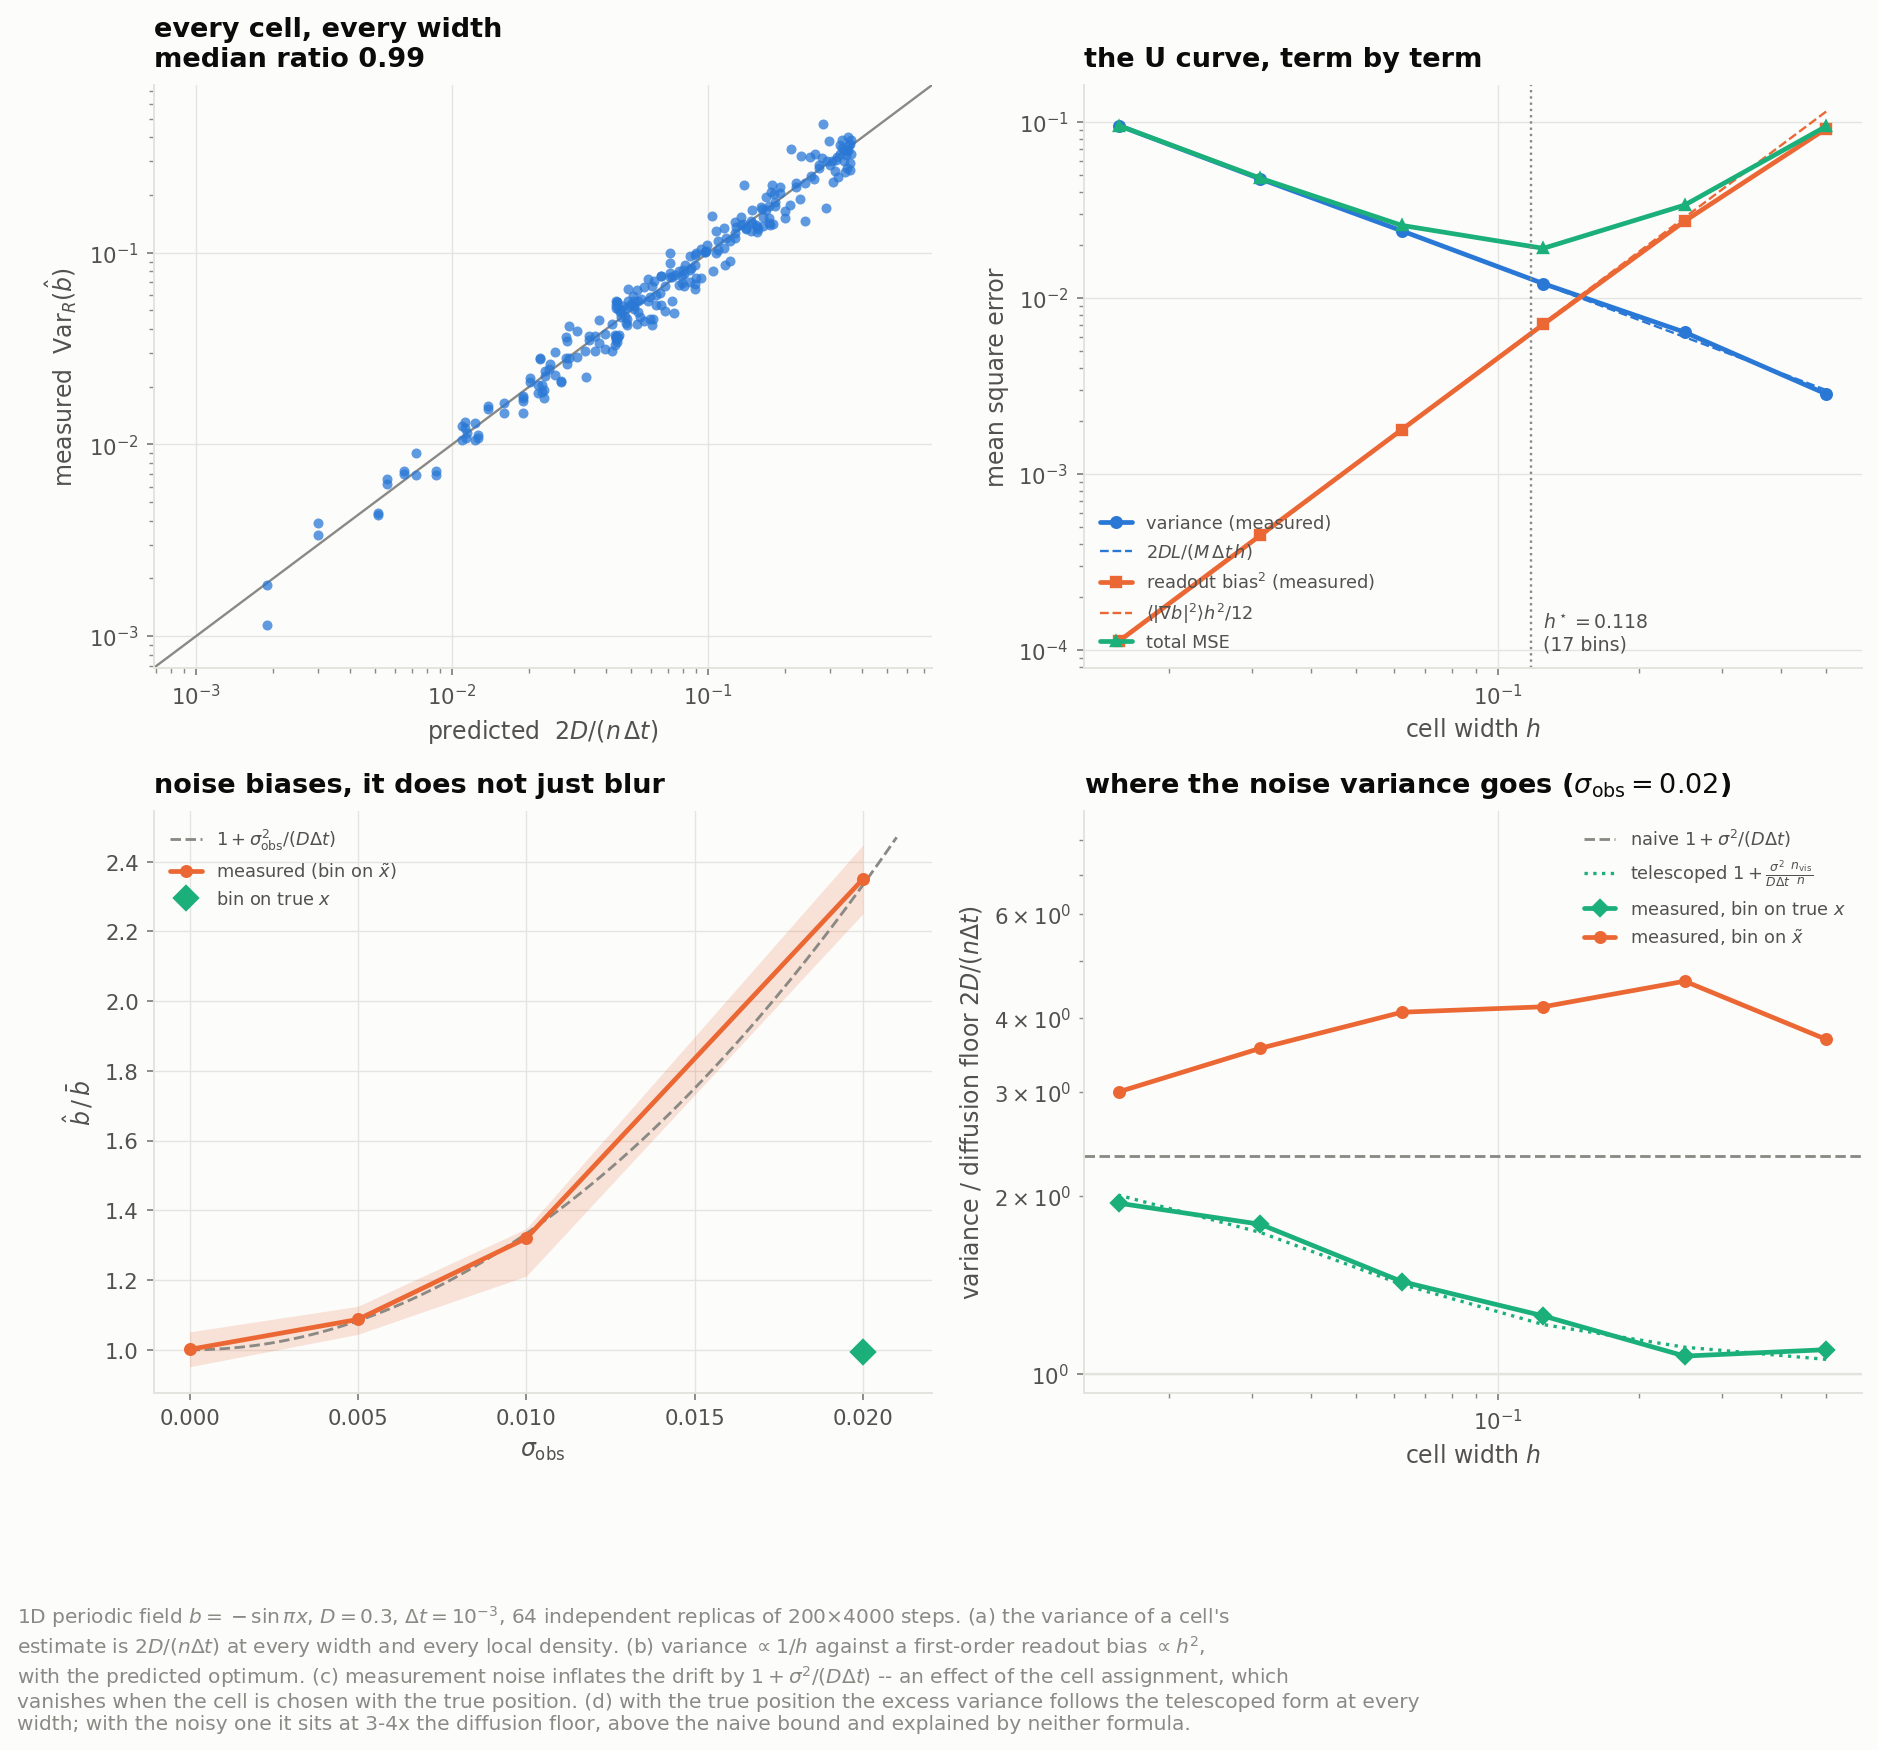
\includegraphics[width=0.99\textwidth]{figs/binned_error_budget.png}
\caption{(a) the variance of a cell's estimate equals $2D/(n\dt)$ at every cell width
and every local density \textemdash{} every point is one cell of one grid, 252 in all.
(b) the two terms of \eqref{eq:total} measured separately against their predictions, and
their sum, with the predicted optimum marked. (c) measurement noise inflates the drift by
$1+\sigma^{2}/(D\dt)$; the green diamond is the control in which the increment is noisy
but the cell is chosen with the true position. (d) the same control across cell widths:
with the true position the excess variance follows the telescoped form \eqref{eq:tele};
with the noisy one it sits at 3\textendash4$\times$ the diffusion floor at every width,
above the naive bound.}
\end{figure}

\subsection{Variance and the U curve}

\begin{center}
\small
\begin{tabular}{@{}rrrrrrr@{}}
\toprule
bins & $h$ & $n$ per cell & $\operatorname{Var}$ measured & $2D/(n\dt)$ &
readout$^2$ measured & $\langle|\nabla b|^{2}\rangle h^{2}/12$ \\
\midrule
  4 & 0.500 & 199\,947 & 0.00285 & 0.00300 & 0.0920 & 0.1150 \\
  8 & 0.250 &  85\,159 & 0.00639 & 0.00600 & 0.0274 & 0.0288 \\
 16 & 0.125 &  39\,708 & 0.01209 & 0.01200 & 0.00709 & 0.00719 \\
 32 & 0.0625 & 19\,436 & 0.02411 & 0.02400 & 0.00179 & 0.00180 \\
 64 & 0.0313 &  9\,665 & 0.04756 & 0.04800 & 0.00045 & 0.00045 \\
128 & 0.0156 &  4\,825 & 0.09557 & 0.09600 & 0.00011 & 0.00011 \\
\bottomrule
\end{tabular}
\end{center}

The per-cell ratio of measured to predicted variance has median $0.97$\textendash$1.09$
across all six widths (0.99 pooled over all 252 cells). The variance doubles at every
halving of $h$, as $h^{-d}$ with $d=1$ demands. The readout bias follows $Bh^{2}$ with
$B=\langle|\nabla b|^{2}\rangle_\rho/12 = 0.460$ to within 1\% for
$h\le0.125$, and falls short at $h=0.5$ where the quadratic approximation to a sine
gives up.

With $M=8\times10^{5}$ this predicts $h^{\star}=0.118$, i.e.\ \textbf{17.0 bins}; the
measured total error is minimised at \textbf{16 bins} (the nearest available). The
optimum is shallow on the fine-grid side and steep on the coarse side, which is the
usual shape: over-smoothing is worse than under-smoothing for a piecewise-constant fit.

\subsection{Measurement noise}

\begin{center}
\small
\begin{tabular}{@{}rrrrrrr@{}}
\toprule
$\sigma_{\mathrm{obs}}$ & $1+\sigma^{2}/(D\dt)$ & measured $\hat b/\bar b$ &
steps per visit & $\frac{\operatorname{Var}}{\text{diffusion only}}$ &
$\frac{\operatorname{Var}}{\text{naive }2\sigma^{2}/n\dt^{2}}$ &
$\frac{\operatorname{Var}}{\text{telescoped}}$ \\
\midrule
0      & 1.000 & 1.001 & 6.3 & 0.97 & 0.97 & 0.97 \\
0.005  & 1.083 & 1.087 & 6.1 & 1.15 & 1.06 & 1.14 \\
0.010  & 1.333 & 1.320 & 5.5 & 1.81 & 1.36 & 1.71 \\
0.020  & 2.333 & 2.350 & 4.1 & 4.18 & 1.79 & 3.17 \\
\midrule
\multicolumn{2}{@{}l}{0.020, cell chosen with the \emph{true} $x$} & 0.993 & 6.3 & 1.25 & 0.54 & 1.03 \\
\bottomrule
\end{tabular}
\end{center}

The inflation formula \eqref{eq:inflation} is confirmed to better than 1.5\% over a
factor of 5 in $\sigma$. The last row is the decisive control: feed the estimator the
same noisy increments but choose the cell with the true position, and

\begin{itemize}[leftmargin=1.2em,itemsep=0.15em]
\item the bias \textbf{vanishes} ($0.993$ instead of $2.350$) \textemdash{} so the damage is
      done by the \emph{binning}, not by the noise in the increment;
\item the variance matches the telescoped formula \eqref{eq:tele} to 3\%, while the naive
      $2\sigma^{2}/(n\dt^{2})$ overestimates it by a factor $1.9$ \textemdash{} telescoping
      is real;
\item with noisy binning the variance is instead $4.2\times$ the diffusion term, and
      panel (d) shows it stays between $3\times$ and $4.4\times$ at every cell width from
      $h=0.016$ to $h=0.5$. Neither formula accounts for it. The mechanism is the same
      selection that produces the bias \textemdash{} near a cell edge, membership and the
      $-\varepsilon_k/\dt$ carried by the increment are correlated \textemdash{} but I
      have no closed form for its size, and the measured width-independence is not what a
      naive edge-fraction argument ($\propto\sigma/h$) would give. It is the one term in
      this note that is measured and not derived.
\end{itemize}

\subsection{Against the project's own sweeps}

An independent check on the 2D random field, from
\code{outputs/local\_study/data/sweep\_obs\_noise.csv} (256 walkers, 4000 steps,
$D=0.3$, three seeds with slightly different stability-chosen $\dt$). Predicted
$\mathrm{nrmse}$ is $\sigma^{2}/(D\dt)$ from \eqref{eq:inflation}, combined in
quadrature with the noise-free error of the same run:

\begin{center}
\small
\begin{tabular}{@{}rrrrr@{}}
\toprule
$\dt$ & $\sigma^{2}/(D\dt)$ at $\sigma=0.02$ & noise-free nrmse & predicted & measured \\
\midrule
$1.051\times10^{-3}$ & 1.268 & 0.446 & 1.344 & 1.486 \\
$0.787\times10^{-3}$ & 1.695 & 0.514 & 1.771 & 1.933 \\
$1.211\times10^{-3}$ & 1.101 & 0.458 & 1.192 & 1.267 \\
\bottomrule
\end{tabular}
\end{center}

Within $7$\textendash$10\%$ across a $1.5\times$ range of $\dt$, in a different
dimension and a different field family, with no fitted constant. The residual is the
edge-selection variance of the previous table, which the prediction omits.

% ==========================================================================
\clearpage
\section{Notes on the handwritten sheet}

\begin{figure}[h]
\centering
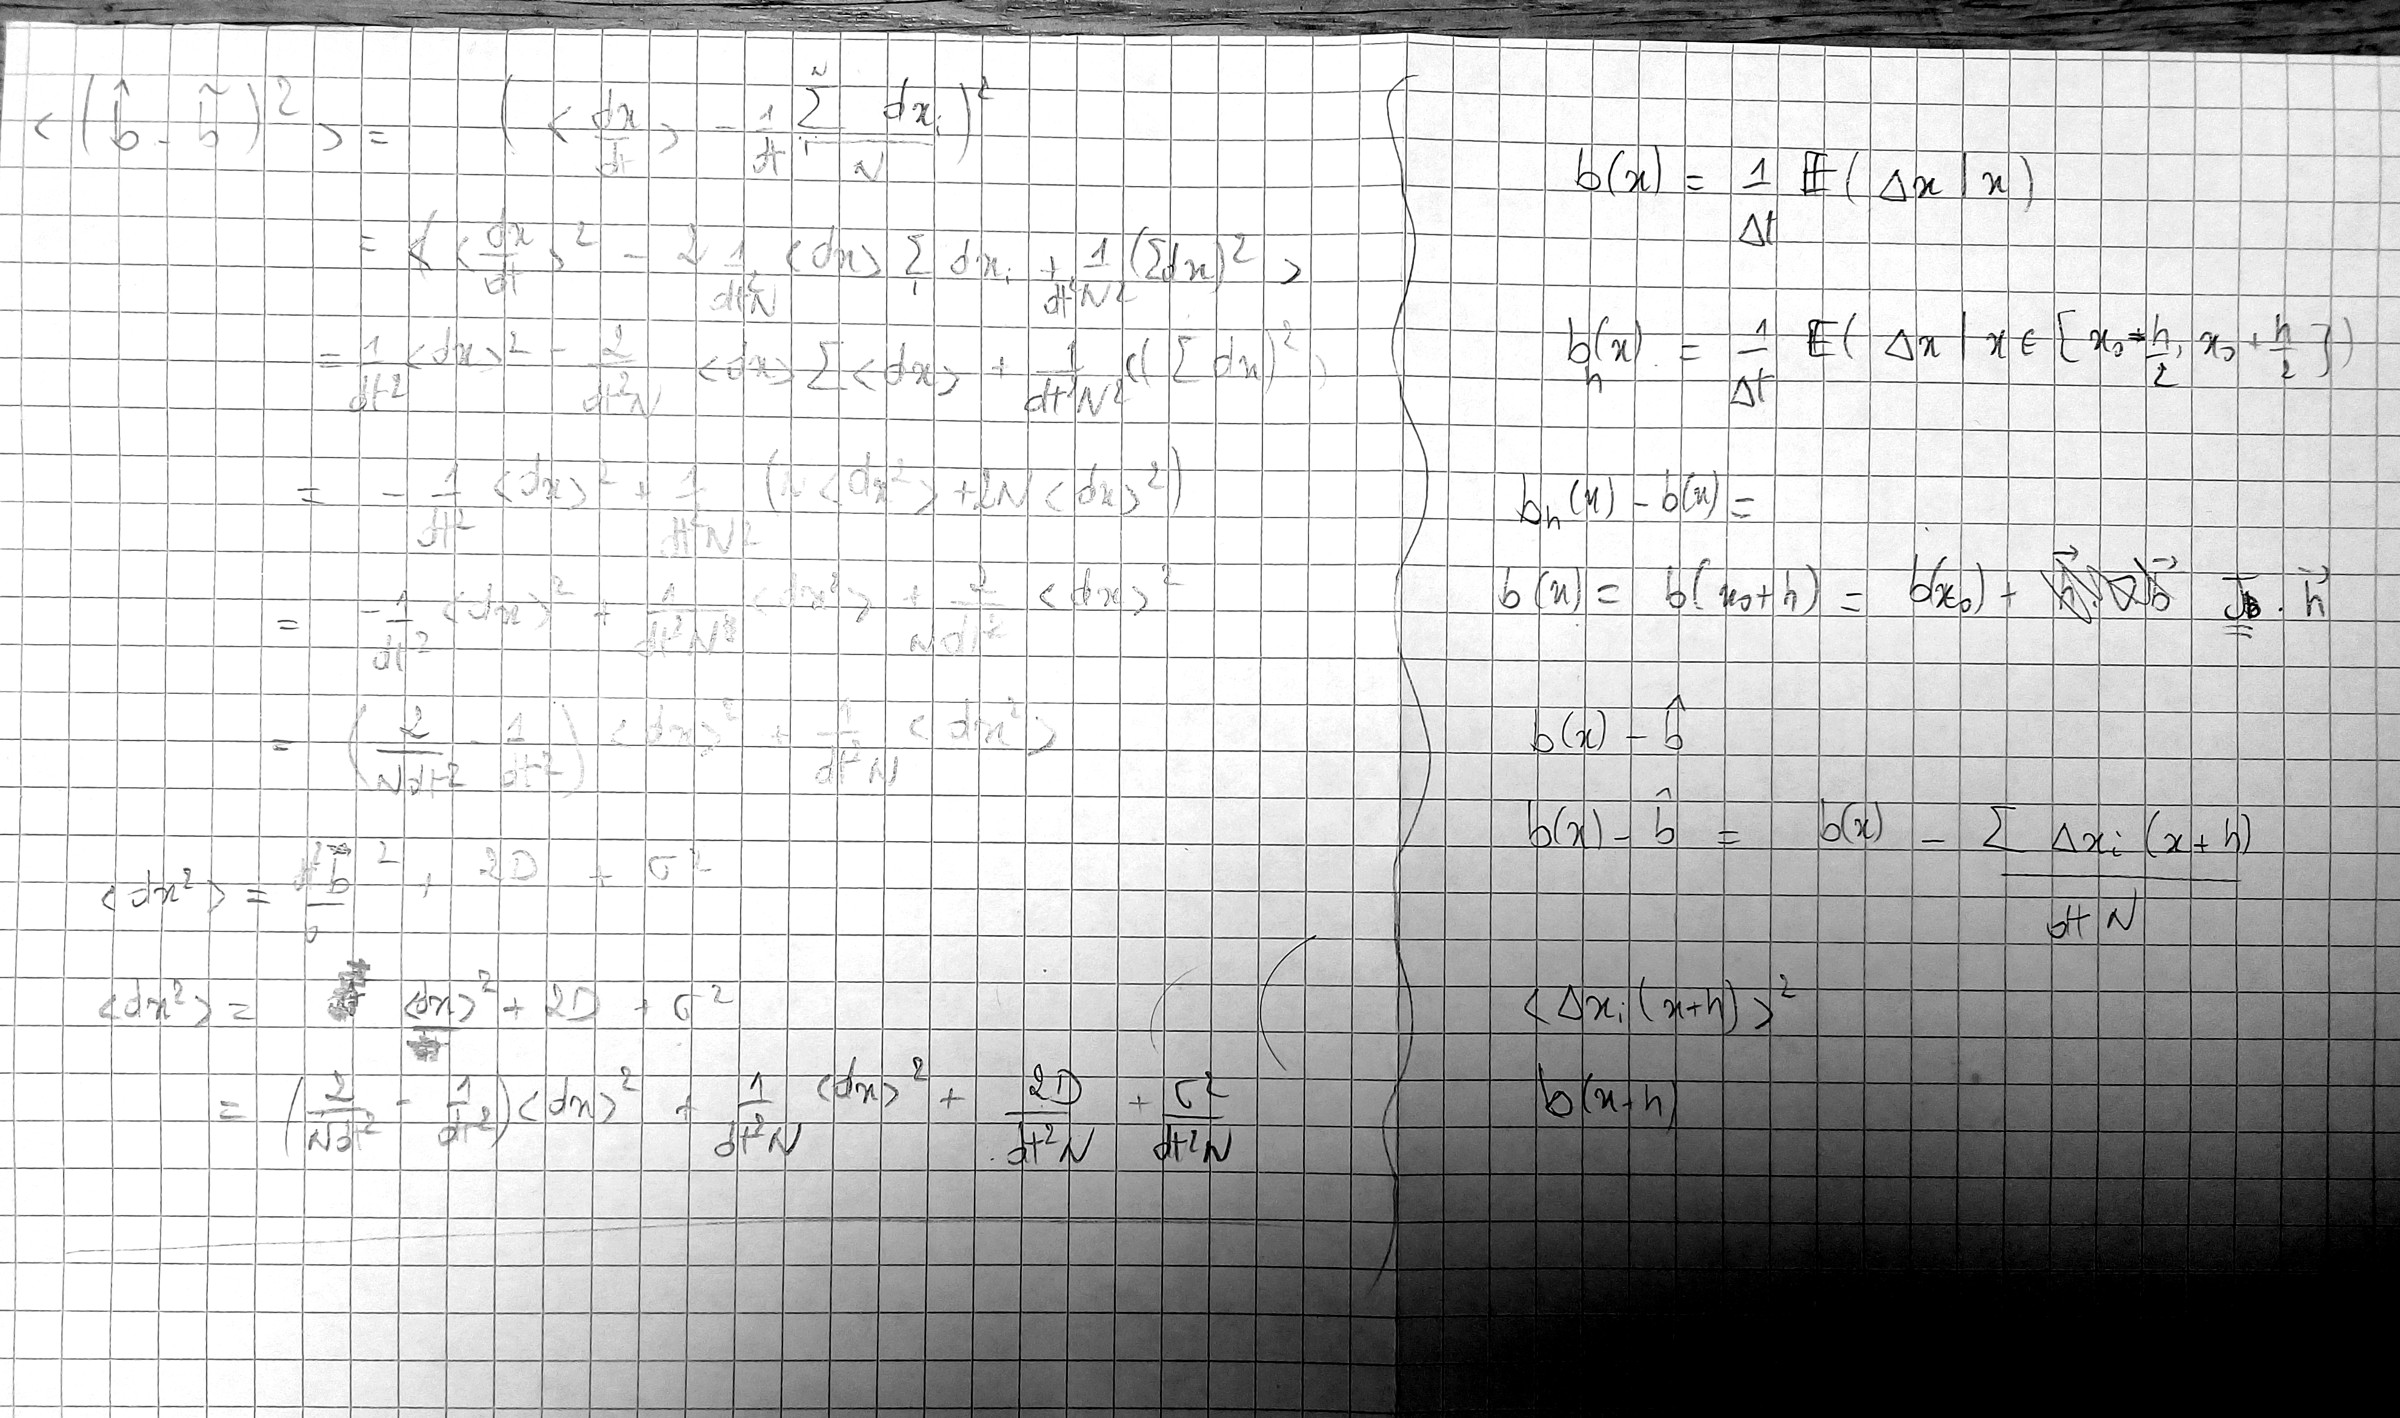
\includegraphics[width=0.94\textwidth]{figs/handwritten_derivation.jpg}
\caption{The draft under discussion. Left column: the variance of the cell mean.
Right column: the bin-width bias.}
\end{figure}

\textbf{What is right.} The structure is the right structure: variance of a sample mean
on the left, a Taylor expansion of $b$ across the cell on the right. The conditional-mean
definition $b(x)=\frac{1}{\dt}\E[\dx\,|\,x]$ and its binned version
$b_h(x)=\frac{1}{\dt}\E[\dx\,|\,x\in[x_0-\tfrac h2,x_0+\tfrac h2]]$ are exactly right,
and so is expanding with the Jacobian, $b(x_0+h)=b(x_0)+J_b\,\vec h$, rather than a
scalar derivative. Reaching a $\frac{1}{N\dt^{2}}\langle\dx^{2}\rangle$-shaped answer
with a $2D$ term and a $\sigma^{2}$ term in it means the skeleton is sound.

The last two lines of the right-hand column,
$b(x)-\hat b = b(x)-\frac{1}{N\dt}\sum_i\dx_i(x+h)$, are the start of exactly the right
move \textemdash{} putting the bias and the estimator into one expression instead of two
separate columns. Carried through, that is \eqref{eq:total}, and it is where the
$h$-dependence of $N$ becomes unavoidable. It is worth finishing.

\subsection*{Six corrections}

\begin{enumerate}[leftmargin=1.5em,itemsep=0.45em]

\item \textbf{$\big(\sum\dx\big)^{2}$: the cross terms are $N(N\!-\!1)$, not $2N$ (nor
$N^{2}$).} The sheet has
$\frac{1}{\dt^{2}N^{2}}\big(N\langle\dx^{2}\rangle+2N\langle\dx\rangle^{2}\big)$;
it should be $\frac{1}{\dt^{2}N^{2}}\big(N\langle\dx^{2}\rangle+N(N\!-\!1)\langle\dx\rangle^{2}\big)$,
as in \eqref{eq:square}. The consequence is visible two lines later: the
$-\frac{1}{\dt^{2}}\langle\dx\rangle^{2}$ from the first line never cancels, and the final
expression still carries $\big(\tfrac{2}{N\dt^{2}}-\tfrac{1}{\dt^{2}}\big)\langle\dx\rangle^{2}$.
That is a term of size $b^{2}$, i.e.\ the \emph{entire drift squared} \textemdash{} not a
small correction, and negative. With the right count everything collapses to
$\operatorname{Var}(\dx)/(N\dt^{2})$ and no $\langle\dx\rangle^{2}$ survives.

\item \textbf{$\langle\dx^{2}\rangle=\langle\dx\rangle^{2}+2D+\sigma^{2}$ is missing a
$\dt$.} It is $2D\dt$: the mean square displacement of a Brownian step grows
\emph{linearly in time}. Dimensionally, $[\dx^{2}]=\mathrm{length}^{2}$ while
$[D]=\mathrm{length}^{2}/\mathrm{time}$. Carried through, the sheet's diffusion term
becomes $\frac{2D}{N\dt^{2}}$ where it should be $\frac{2D}{N\dt}$ \textemdash{} a
factor $\dt$, which at $\dt=10^{-3}$ is a factor of a thousand in the variance, and it
is the term that decides everything.

\item \textbf{The measurement-noise term is $2\sigma^{2}$, not $\sigma^{2}$.} The
observed increment is $\dx+\varepsilon_{k+1}-\varepsilon_k$, a \emph{difference} of two
independent draws \eqref{eq:noisyinc}. And even $2\sigma^{2}$ per increment is too many:
consecutive steps inside a cell telescope, leaving $2\sigma^{2}$ per \emph{visit}
\eqref{eq:tele}, which at these settings is a further factor of $\approx6$.
Measured: the naive form overestimates by $1.9\times$, the telescoped form is exact to 3\%.

\item \textbf{$h$ never appears in the variance, because $N$ is carried as a free symbol.}
This is the structural gap, not an algebra slip. $N=M\rho h^{d}$ is the \emph{only} way
$h$ reaches the variance, and without it there is no tradeoff against the bias on the
right-hand column, no optimal cell width, and no way to answer ``how many bins?''.
The two columns of the sheet are the two halves of \eqref{eq:total} and they need to be
added, in the same variables.

\item \textbf{$\dt$ cancels in the diffusion term and does not cancel in the noise term.}
Substituting $N=M\rho h^{d}$ turns $\frac{2D}{N\dt}$ into $\frac{2D}{M\rho h^{d}\dt}$,
which at fixed \emph{total time} $M\dt$ is independent of the sampling rate, while
$\frac{2\sigma^{2}}{N\dt^{2}}$ still carries one power of $1/\dt$. The sheet treats both
as $\frac{1}{N\dt^{2}}$-type terms with $N$ independent of $\dt$, which hides the single
asymmetry that decides how fast one should sample.

\item \textbf{$\sigma_{\mathrm{obs}}$ appears only in the variance, and its main effect
is a bias.} At $\sigma=0.02$ the inflation \eqref{eq:inflation} contributes $1.33$ to the
nrmse on its own, against $0.4$\textendash$0.8$ from the extra variance (the quadrature
residuals in \S6.3). Both matter; only one of the two is in the sheet, and it is the
smaller. The mechanism is not in
the sheet's model at all, because the sheet conditions on the \emph{true} cell membership:
the damage comes from the cell being chosen with $\tilde x$. That is the difference
between the last two rows of the table on the previous page \textemdash{} $0.993$ versus
$2.350$ \textemdash{} and it is the whole story of why the snapshot methods win at
$\sigma_{\mathrm{obs}}=0.02$ while every trajectory method in the ladder collapses.

\end{enumerate}

\subsection*{Two things simply not there}

\begin{itemize}[leftmargin=1.5em,itemsep=0.25em]
\item The $O(\dt)$ discretisation bias $\frac{\dt}{2}[(b\!\cdot\!\nabla)b+D\nabla^{2}b]$,
      which is independent of $N$, $h$ and $\sigma$ and sets the floor at large $\dt$.
\item The factor $d$: in $d$ dimensions $\E|\hat b-b|^{2}=\frac{2dD}{N\dt}+\dots$,
      since each component carries its own noise.
\end{itemize}

\subsection*{One refinement on the right-hand column, which is otherwise correct}

$b_h-b\simeq J_b\vec h$ is the right leading term \emph{for this estimator}, and it is
worth being precise about why. Averaged over the cell, $\bar b_C$ is accurate to
$O(h^{2})$: the linear term cancels because the cell is symmetric about $x_0$. The first
order survives only because the estimator is asked for $b$ at a query point
$x=x_0+\delta$ and answers with the cell's single value. So the right statement is
\eqref{eq:readout}: the displacement is $\delta$, uniform over the cell, giving
$|\nabla b|^{2}h^{2}/12$ rather than $|\nabla b|^{2}h^{2}$. The factor $1/12$ matters:
with it $h^{\star}$ is 17 bins, which is what the measurement shows; without it, 39.

\begin{keybox}
This distinction is exactly the gap that rung 2 collects. A kernel centred on the query
point has no displacement to pay for, so its bias is $O(h^{2})$ everywhere: log-log
slope 1.85 measured, against 0.97 for the grid. It is also why the two estimators want
different bin-count rules, $M^{1/(d+2)}$ against $M^{1/(d+4)}$.
\end{keybox}

% ==========================================================================
\section{The whole budget, assembled}

\begin{center}
\small
\begin{tabular}{@{}L{0.30\textwidth} L{0.30\textwidth} L{0.32\textwidth}@{}}
\toprule
\textbf{term} & \textbf{size} & \textbf{what changes it} \\
\midrule
statistical variance & $\dfrac{2dD}{M\rho h^{d}\dt}=\dfrac{2dD}{T_{\mathrm{occ}}}$ &
more walkers, longer runs, wider cells, smaller $D$. \emph{Not} the sampling rate. \\
readout bias & $\dfrac{|\nabla b|^{2}h^{2}}{12}$ &
narrower cells; or a kernel, which has $O(h^{2})$ bias, i.e.\ $O(h^{4})$ here \\
discretisation bias & $\dfrac{\dt}{2}\big[(b\!\cdot\!\nabla)b+D\nabla^{2}b\big]$ &
sampling faster \textemdash{} the only term that wants small $\dt$ \\
noise variance & $\dfrac{2\sigma^{2}n_{\mathrm{vis}}}{n^{2}\dt^{2}}$ &
sampling \emph{slower}; wider cells (more telescoping) \\
noise bias & $b\,\dfrac{\sigma^{2}}{D\dt}$ &
sampling slower; better metrology. No amount of data helps \\
\bottomrule
\end{tabular}
\end{center}

Reading the table as an experimental design: $\dt$ is pulled down by the discretisation
bias and pushed up, far harder, by everything involving $\sigma_{\mathrm{obs}}$; $h$ is
pulled down by the readout bias and up by the variance, balancing at
$M^{1/(d+2)}$ bins per axis; and $M$ buys error only as $M^{-1/(d+2)}$, which is why
the ladder does not stop at rung 1.

\end{document}
